\newpage

\subsection{Database Schema}

\begin{figure}[H]
  \centering
  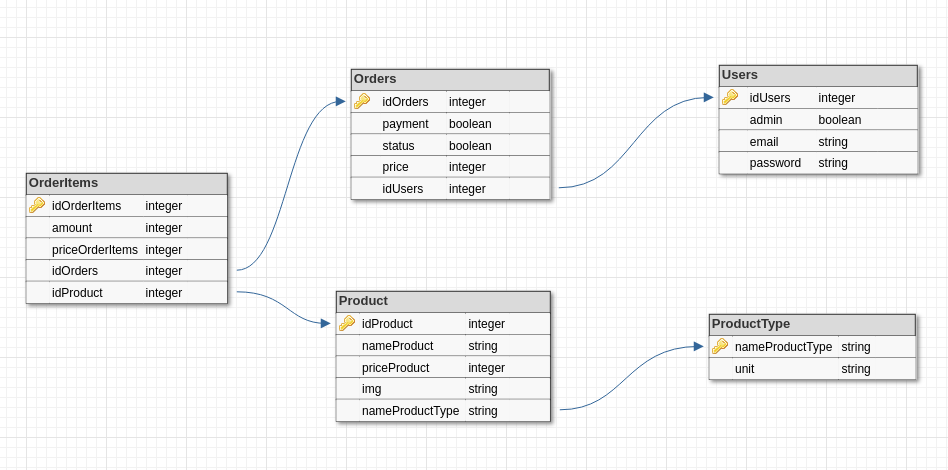
\includegraphics[width=\textwidth]{second_sprint/db_schema.png}
  \caption{\label{fig:schema} The database schema.}
\end{figure}

\begin{itemize}
  \item[\textbf{Users:}] Contains the users, both admins and non-admins. The
    email is used to identify user at login, so no username is needed.
  \item[\textbf{Orders:}] Contains an order. This is used to represent
    the shopping basket before an order was made 
    (\mintinline{python}{payment == false}) an order that has been paid but not 
    yet processed and shipped 
    (\mintinline{python}{payment == True and status == False}), as well as
    finished orders (\mintinline{python}{status == True}). Each order has
    one user.
  \item[\textbf{OrderItems:}] The items of an order with foreign keys
    idOrders and idProduct to the tables Orders and Product.  Keeps the
    amount, price and id of a product in an order.
  \item[\textbf{Product:}] Foreign keys idBerry and idGoods to the tables
    Berry and Goods.
  \item[\textbf{ProductType:}] Foreign key idBerryType to table BerryType. Contains
    name of berry.
\end{itemize}
